\section{Terrain Generation}

The very first option in the application is to generate the terrain. It creates a mesh of triangles that will be given a certain height value from a noise map. Some variables that affect the terrain terrain can be adjusted by the user, those options being:

\begin{easylist}
 @ Sea level: increase or decrease the water level
 @ Offset X and Z: slide along the respective axis in the noise map, changing the height values of the terrain.
 @ Size X and Z: Adjust the size of the entire terrain.
\end{easylist}


\begin{figure}[h!]
  \centering

  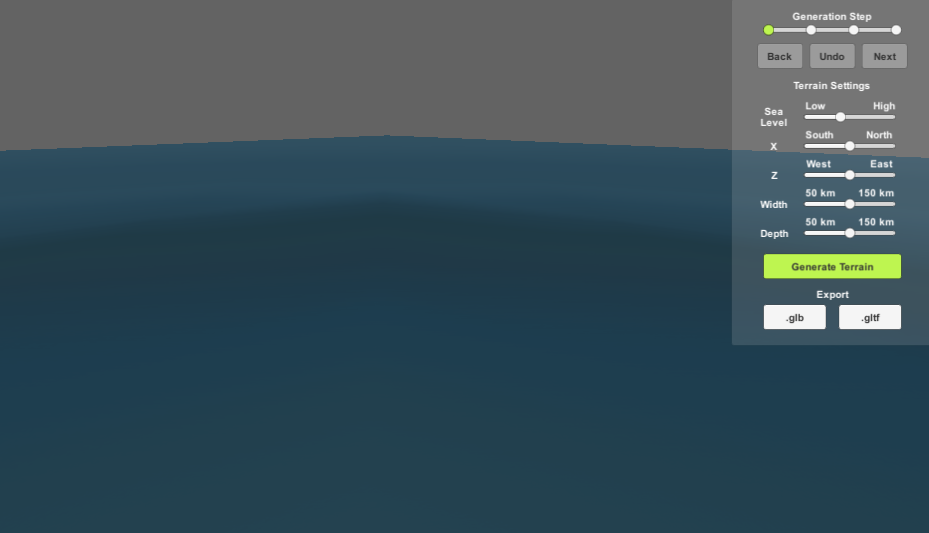
\includegraphics[width=0.8\textwidth]{figure/terrain_not_generated.png}
  \caption{The state before Generate Terrain button has been pressed. The water is visible from the very beginning.}

  \label{fig:no_terr}
\end{figure}

\begin{figure}[h!]
  \centering

  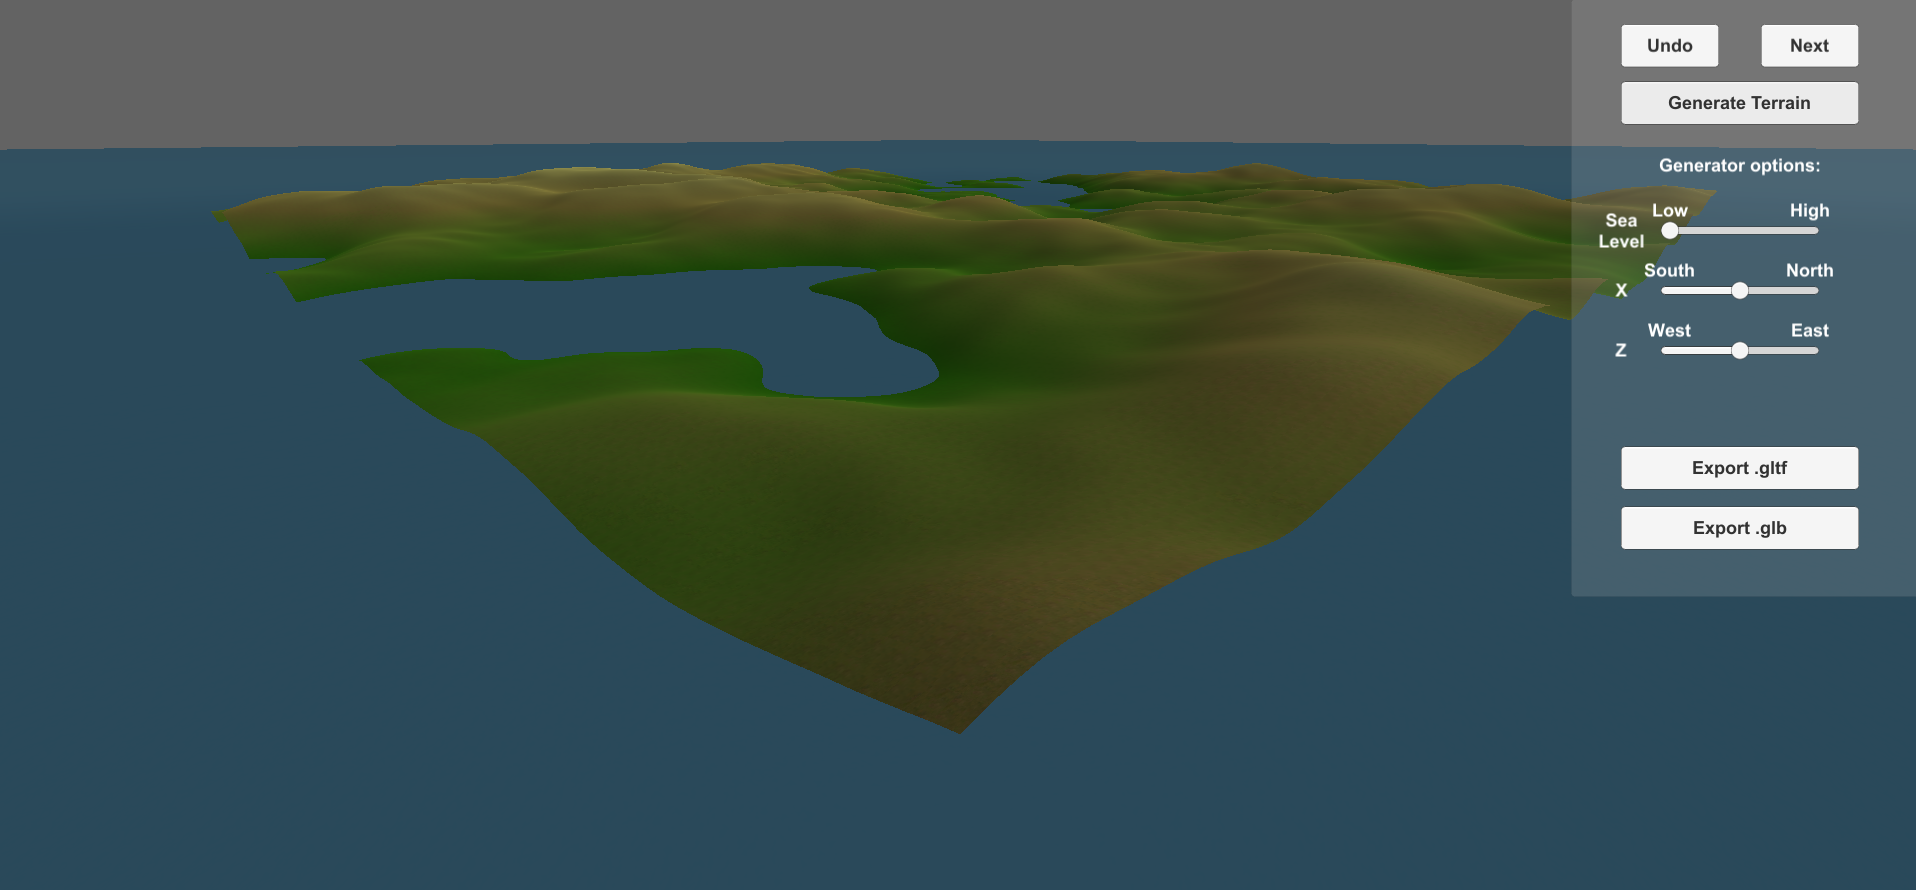
\includegraphics[width=0.8\textwidth]{figure/terrain_generated.png}
  \caption{The state after Generate Terrain button has been pressed.}

  \label{fig:terr}
\end{figure}
